\documentclass[aspectratio=169,11pt]{beamer}

% ================================================================
% "TABIIY TILNI QAYTA ISHLASH" KURSI
% MA'RUZA 11 --- Neyron mashina tarjimasi: Seq2Seq va Attention
%              (d11_seq2seq_attention.tex)
% Arxetiplar: [A][B][C][D][E] + 4 tsikl [F][G][H][I][J][K][L] +
%             [M][N][O][P][Q][R] + ilova [S]
% Rendered slayd soni: ~45 (3-haftaning uchinchi ma'ruzasi; L1-L10 chuqurligi)
% Qulflangan [I3]: attention alpha = softmax([2,1,3]) = [0.245, 0.090, 0.665]
%   --- P11 (Day 12) birinchi assert manbayi (course_map hand_example).
% ================================================================

% ================================================================
% RANGLAR  (asl fayldan o'zgarishsiz)
% ================================================================
\definecolor{cnublue}{rgb}{0.07,0.14,0.62}
\definecolor{cnubluelight}{rgb}{0.18,0.30,0.72}
\definecolor{cnubluebg}{rgb}{0.90,0.92,0.97}
\definecolor{deepblue}{rgb}{0.07,0.14,0.62}
\definecolor{deepred}{rgb}{0.60,0.00,0.00}
\definecolor{deepgreen}{rgb}{0.00,0.45,0.00}
\definecolor{halfgray}{gray}{0.55}

% ================================================================
% BEAMER MAVZU --- Boadilla + maxsus footer  (asl fayldan o'zgarishsiz)
% ================================================================
\usetheme{Boadilla}

\setbeamercolor{structure}{fg=cnublue}
\setbeamercolor{frametitle}{bg=cnublue,fg=white}
\setbeamercolor{title}{bg=cnublue,fg=white}
\setbeamercolor{block title}{bg=cnublue,fg=white}
\setbeamercolor{block body}{bg=cnubluebg,fg=black}
\setbeamercolor{alerted text}{fg=deepred}
\setbeamercolor{author in head/foot}{bg=cnubluelight,fg=white}
\setbeamercolor{section in head/foot}{bg=cnublue,fg=white}
\setbeamercolor{page number in head/foot}{bg=cnubluelight,fg=white}

\setbeamertemplate{mini frame}{}
\setbeamertemplate{mini frame in current section}{}
\setbeamertemplate{mini frame in current subsection}{}
\setbeamertemplate{headline}{}
\setbeamertemplate{navigation symbols}{}

\setbeamertemplate{footline}{%
  \leavevmode%
  \hbox{%
    \begin{beamercolorbox}[wd=0.17\paperwidth,ht=2.5ex,dp=1.25ex,leftskip=0.5em]{author in head/foot}%
      \usebeamerfont{author in head/foot}\scriptsize\insertshortauthor%
    \end{beamercolorbox}%
    \begin{beamercolorbox}[wd=0.69\paperwidth,ht=2.5ex,dp=1.25ex,center]{section in head/foot}%
      \usebeamerfont{section in head/foot}%
      \scriptsize\insertsectionnavigationhorizontal{0.69\paperwidth}{}{}%
    \end{beamercolorbox}%
    \begin{beamercolorbox}[wd=0.14\paperwidth,ht=2.5ex,dp=1.25ex,rightskip=0.5em]{page number in head/foot}%
      \hfill\scriptsize\color{white}%
      \insertframenumber{}/\inserttotalframenumber%
    \end{beamercolorbox}%
  }%
  \vskip0pt%
}

% ================================================================
% PAKETLAR  (asl fayldan o'zgarishsiz)
% ================================================================
\usepackage[utf8]{inputenc}
\usepackage[T1]{fontenc}
\usepackage{lmodern}
\usepackage{amsmath,amssymb}
\usepackage{booktabs}
\usepackage{xcolor}
\usepackage{listings}
\lstset{
    language=Python,
    basicstyle=\ttfamily\scriptsize,
    keywordstyle=\bfseries\color{deepblue},
    emphstyle=\ttfamily\color{deepred},
    stringstyle=\color{deepgreen},
    commentstyle=\itshape\color{halfgray},
    numbers=left,
    numberstyle=\scriptsize\color{halfgray},
    rulesepcolor=\color{cnublue!30},
    frame=shadowbox,
    breaklines=true,
    showstringspaces=false,
    tabsize=2
}
\usepackage{tcolorbox}
\tcbuselibrary{skins}
\tcbset{
  defbox/.style={colback=cnubluebg,colframe=cnublue,
                 fonttitle=\small\bfseries\color{white},
                 attach boxed title to top left={yshift=-2mm,xshift=4mm},
                 boxed title style={colback=cnublue,colframe=cnublue}},
  warnbox/.style={colback=orange!8,colframe=orange!70!black,
                  fonttitle=\small\bfseries},
  okbox/.style={colback=green!7,colframe=green!55!black,
                fonttitle=\small\bfseries}
}
\usepackage{tikz}
\usetikzlibrary{arrows.meta,positioning}

% ================================================================
% QO'SHIMCHALAR  (asl fayldan o'zgarishsiz)
% ================================================================
\AtBeginSection[]{%
  \begin{frame}{Prezentatsiya rejasi}
    \tableofcontents[currentsection]
  \end{frame}}

\newcommand{\bunda}[1]{{\small\textbf{bunda:}\; #1}}
\newcommand{\bajarildi}{{\color{deepgreen}\large$\checkmark$}\;}

% ================================================================
% METAMA'LUMOT
% ================================================================
\title[Seq2Seq va Attention]{Neyron mashina tarjimasi: Seq2Seq va Attention}
\subtitle{Tabiiy tilni qayta ishlash --- 11-ma'ruza}
\author[A.A.\,Abdulali]{A.A.\,Abdulali}
\date{2-iyul 2026}
\institute{11:00--12:20 \quad$\cdot$\quad mavzu \textnumero{}11}

% ================================================================
\begin{document}
% ================================================================

% ----------------------------------------------------------------
% [A] TITUL
% ----------------------------------------------------------------
\maketitle

% ================================================================
\section[Kirish]{Kirish: bir tildan boshqasiga tarjima qilamiz}
% ================================================================

% ----------------------------------------------------------------
% [B] TAKRORLASH: L9/L10 va bugungi P10
% ----------------------------------------------------------------
\begin{frame}{Takrorlash: o'tgan darslardan ikki savol}
  \begin{columns}[T]
    \begin{column}{0.49\textwidth}
      \begin{tcolorbox}[warnbox,title=1-savol]
        \small
        L9--L10 da LSTM butun gapni ketma-ket o'qib, oxirgi holat $h_T$ da uni
        "jamladi". Tarjimada manba gapni qanday eslab qolamiz?
      \end{tcolorbox}
    \end{column}
    \begin{column}{0.49\textwidth}
      \begin{tcolorbox}[warnbox,title=2-savol]
        \small
        Butun gapni \textbf{bitta} vektorga siqsak, uzun gapda nima yo'qoladi?
      \end{tcolorbox}
    \end{column}
  \end{columns}
  \pause
  \vspace{4pt}
  \begin{columns}[T]
    \begin{column}{0.49\textwidth}
      \begin{tcolorbox}[okbox,title=1-javob]
        \small
        Enkoder LSTM manbani $h_T$ ga jamlaydi, dekoder LSTM undan tarjima yaratadi
        (enkoder-dekoder). Bugun shu arxitekturani quramiz.
      \end{tcolorbox}
    \end{column}
    \begin{column}{0.49\textwidth}
      \begin{tcolorbox}[okbox,title=2-javob]
        \small
        Boshlang'ich so'zlar "yuviladi" --- \textbf{information bottleneck}. Yechim:
        \textbf{attention} (har qadamda manbaga qaytib qarash).
      \end{tcolorbox}
    \end{column}
  \end{columns}
\end{frame}

% ----------------------------------------------------------------
% [C] MAQSADLAR
% ----------------------------------------------------------------
\begin{frame}{Siz bugungi dars oxirida quyidagilarni bajara olasiz:}
  \begin{enumerate}\setlength\itemsep{6pt}
    \item \textbf{Tushuntira olasiz:} enkoder-dekoder arxitekturasi va uning
          information bottleneck muammosini.
    \item \textbf{Tushuntira olasiz:} attention --- dekoder har qadamda manba
          so'zlariga "qarab" oladi.
    \item \textbf{Hisoblay olasiz:} attention vaznlarini ---
          $\alpha=\mathrm{softmax}([2,1,3])=[0.245,0.090,0.665]$ va kontekst vektorini.
    \item \textbf{Hisoblay olasiz:} tarjima sifatini BLEU bilan.
  \end{enumerate}
  \vspace{4pt}
  \begin{tcolorbox}[defbox,title=Oldindan talab]
    \footnotesize
    L7--L10 dan: LSTM, Bi-LSTM, ketma-ketlik. L6/L9 dan: softmax. Matematikadan:
    skalyar ko'paytma, vaznlangan yig'indi, $\exp$.
  \end{tcolorbox}
\end{frame}

% ----------------------------------------------------------------
% [D] REJA
% ----------------------------------------------------------------
\begin{frame}{Bugungi dars rejasi:}
  \begin{center}
  \small
  \begin{tabular}{c p{5.0cm} c p{3.0cm}}
    \toprule
    \textbf{Tsikl}& \textbf{Mavzu} & \textbf{Vaqt} & \textbf{Hosil bo'luvchi natija}\\
    \midrule
    1 & Enkoder-Dekoder va bottleneck & 16 daq & sobit kontekst muammosi \\
    2 & Attention: ortga qarash & 16 daq & har qadam yangi kontekst \\
    3 & Attention hisoblash (Q/K/V) & 18 daq & $\alpha=[0.245,0.090,0.665]$ \\
    4 & BLEU bilan baholash & 16 daq & BLEU-1 $=0.667$ \\
    \midrule
      & Xulosa va 11-amaliyotga ko'rsatmalar & 10 daq & Ertaga nima qurishingiz \\
    \bottomrule
  \end{tabular}
  \end{center}
  \vspace{4pt}
  \begin{tcolorbox}[warnbox,title=Bu dars attention'ga olib keladi]
    \footnotesize\sloppy
    Enkoder-dekoder bottleneck'ini attention bilan yechamiz. Bugungi
    $\alpha=[0.245,0.090,0.665]$ ertangi P11 da \texttt{assert} bo'ladi.
  \end{tcolorbox}
\end{frame}

% ----------------------------------------------------------------
% [E] MUAMMO BIRINCHI
% ----------------------------------------------------------------
\begin{frame}{Bugungi dars uchun muammo: uzun gapni bitta vektorga sig'dirib bo'lmaydi}
  \begin{columns}[T]
    \begin{column}{0.50\textwidth}
      \textbf{Sodda yechim qayerda qiynaladi:}\\[3pt]
      \small
      \begin{tcolorbox}[warnbox,title={Sobit kontekst vektori},top=2pt,bottom=2pt]
        \footnotesize
        Enkoder butun manba gapni \textbf{bitta} $h_T$ vektoriga siqadi. Dekoder
        faqat shunga tayanadi.
      \end{tcolorbox}
      \vspace{3pt}
      \begin{tcolorbox}[warnbox,title={Uzun gap = ko'p yo'qotish},top=2pt,bottom=2pt]
        \footnotesize
        Gap uzunlashgani sari boshidagi so'zlar axboroti "yuviladi" --- tarjima
        sifati tushadi.
      \end{tcolorbox}
    \end{column}
    \begin{column}{0.46\textwidth}
      \textbf{Bugungi yechim:}\\[4pt]
      \small
      \begin{enumerate}\setlength\itemsep{4pt}
        \item Enkoder \textbf{har} so'z uchun holat saqlaydi ($h_1\ldots h_n$).
        \item Dekoder har qadamda \textbf{kerakli} manba so'zlariga qaraydi.
        \item Bu "qarash" --- vaznlangan yig'indi (\textbf{attention}).
      \end{enumerate}
      \vspace{5pt}
      \begin{tcolorbox}[okbox,top=2pt,bottom=2pt]
        \footnotesize
        Bahdanau attention: dekoderga manbaning \textbf{tegishli} qismini har qadam
        tanlash imkonini beradi.
      \end{tcolorbox}
    \end{column}
  \end{columns}
\end{frame}

% ================================================================
\section[Enkoder-Dekoder]{Enkoder-Dekoder va bottleneck}
% ================================================================

% ----------------------------------------------------------------
% [F1] INTUITSIYA
% ----------------------------------------------------------------
\begin{frame}{Intuitsiya: o'qi, jamla, keyin yoz}
  \begin{columns}[T]
    \begin{column}{0.52\textwidth}
      \small
      Tarjima ikki bosqich:
      \begin{itemize}\setlength\itemsep{1pt}
        \item \textbf{Enkoder} (LSTM): manba gapni o'qiydi, ma'noni $h_T$ ga jamlaydi.
        \item \textbf{Dekoder} (LSTM): $h_T$ dan boshlab, maqsad tilda so'zma-so'z
              yozadi (autoregressiv, L9).
      \end{itemize}
      \vspace{4pt}
      \texttt{[men kitob o'qidim]} $\to h_T \to$ \texttt{[I read a book]}.
    \end{column}
    \begin{column}{0.44\textwidth}
      \begin{tcolorbox}[okbox,top=2pt,bottom=2pt]
        \footnotesize
        Muammo: $h_T$ --- \textbf{bitta} sobit vektor. Butun gap ma'nosi shunga
        sig'ishi kerak --- uzun gapda bu yetmaydi (bottleneck).
      \end{tcolorbox}
    \end{column}
  \end{columns}
\end{frame}

% ----------------------------------------------------------------
% [G1] RASMIY TA'RIF + BUNDA
% ----------------------------------------------------------------
\begin{frame}{Enkoder-Dekoder: rasmiy ta'rif}
  \begin{tcolorbox}[defbox,title=Ta'rif: Seq2Seq (attention'siz)]
    \vspace{-0.4em}
    $$ \mathbf{c} = h_n^{\text{enc}}, \qquad
       s_t = \mathrm{LSTM}_{\text{dec}}(s_{t-1}, [y_{t-1}; \mathbf{c}]), \qquad
       \hat{y}_t = \mathrm{softmax}(W s_t) $$
  \end{tcolorbox}
  \vspace{2pt}
  \bunda{$h_n^{\text{enc}}$ --- enkoderning oxirgi holati (kontekst $\mathbf{c}$);
  $s_t$ --- dekoder holati; $y_{t-1}$ --- oldingi maqsad so'z; $\hat{y}_t$ ---
  $t$ qadamdagi so'z taqsimoti.}
  \vspace{4pt}
  \footnotesize Diqqat: $\mathbf{c}$ \textbf{barcha} dekoder qadamlari uchun
  \textbf{bir xil} --- mana shu bottleneck.
\end{frame}

% ----------------------------------------------------------------
% [H1] KELTIRIB CHIQARISH
% ----------------------------------------------------------------
\begin{frame}{Keltirib chiqarish: nega sobit kontekst yetmaydi?}
  \textbf{1-qadam.} Butun manba gap ma'nosi $\mathbf{c}=h_n$ ga kodlanadi ---
  o'lcham sobit (masalan 512).
  \pause
  \textbf{2-qadam.} Gap uzunlashsa ham $\mathbf{c}$ o'lchami o'zgarmaydi $\Rightarrow$
  axborot \textbf{zichlashadi}, boshidagi so'zlar yo'qoladi.
  \pause
  \textbf{3-qadam.} Dekoder har qadamda bir xil $\mathbf{c}$ ni ko'radi --- qaysi
  manba so'zi hozir muhimligini \textbf{ajrata olmaydi}.
  \begin{tcolorbox}[okbox,top=2pt,bottom=2pt]
    \small \textbf{Xulosa:} kerak bo'lgani --- har dekoder qadami uchun
    \textbf{boshqa}, tegishli kontekst. Buni attention beradi.
  \end{tcolorbox}
\end{frame}

% ----------------------------------------------------------------
% [I1] QO'LDA MISOL
% ----------------------------------------------------------------
\begin{frame}{Qo'lda misol: sobit kontekst axborotni yo'qotadi}
  \begin{tcolorbox}[defbox,title={Enkoder holatlari (o'lcham 2)}]
    \small $h_1=[1,0]$ (men), $h_2=[0,1]$ (kitob), $h_3=[1,1]$ (o'qidim).
  \end{tcolorbox}
  \vspace{0.2em}
  \begin{columns}[T]
    \begin{column}{0.52\textwidth}
      \textbf{Attention'siz kontekst:}
      $$ \mathbf{c} = h_3 = [1, 1] $$
      Dekoder faqat $h_3$ ni ko'radi; $h_1$ (men), $h_2$ (kitob) bevosita yo'q.
    \end{column}
    \begin{column}{0.44\textwidth}
      \begin{tcolorbox}[okbox,top=2pt,bottom=2pt]
        \footnotesize
        Agar dekoder "men" ni tarjima qilmoqchi bo'lsa, unga $h_1$ kerak --- ammo
        sobit $\mathbf{c}=h_3$ uni bevosita bermaydi.
      \end{tcolorbox}
    \end{column}
  \end{columns}
\end{frame}

% ----------------------------------------------------------------
% [J1] SIZNING VAZIFANGIZ
% ----------------------------------------------------------------
\begin{frame}{Sizning vazifangiz: o'rtacha kontekst}
  \begin{tcolorbox}[warnbox,title=Savol --- 60 soniya]
    \small
    Ba'zan kontekst sifatida \textbf{o'rtacha} olinadi: $h_1=[1,0]$, $h_2=[0,1]$,
    $h_3=[1,1]$.\\[4pt]
    \textbf{\large $\mathbf{c}_{\text{avg}} = \tfrac{1}{3}(h_1+h_2+h_3) = ?$}
  \end{tcolorbox}
  \pause
  \begin{tcolorbox}[okbox,title=Javob]
    \small
    $\mathbf{c}_{\text{avg}} = \tfrac{1}{3}([1,0]+[0,1]+[1,1]) = \tfrac{1}{3}[2,2]
       = [0.667, 0.667]$\\[3pt]
    \footnotesize O'rtacha ham sobit va \textbf{teng} vazn beradi --- qaysi so'z
    muhimligini ajratmaydi. Attention esa \textbf{har xil} vazn beradi (3-tsikl).
  \end{tcolorbox}
\end{frame}

% ----------------------------------------------------------------
% [K1] KOD <-> FORMULA  [fragile]
% ----------------------------------------------------------------
\begin{frame}[fragile]{Kod $\leftrightarrow$ formula: enkoder-dekoder skeleti}
  \begin{columns}[T]
    \begin{column}{0.58\textwidth}
\begin{lstlisting}
import torch.nn as nn

class Seq2Seq(nn.Module):
    def __init__(self, src_v, tgt_v, dim, hid):
        super().__init__()
        self.enc = nn.LSTM(dim, hid, batch_first=True)
        self.dec = nn.LSTM(dim, hid, batch_first=True)
        self.emb_s = nn.Embedding(src_v, dim)
        self.emb_t = nn.Embedding(tgt_v, dim)
        self.out = nn.Linear(hid, tgt_v)

    def encode(self, x):
        _, (h, c) = self.enc(self.emb_s(x))
        return h, c    # kontekst (sobit)
\end{lstlisting}
    \end{column}
    \begin{column}{0.38\textwidth}
      \textbf{Kod $\to$ formula:}\\[3pt]
      \footnotesize
      \begin{tabular}{p{1.7cm}p{1.9cm}}
        \toprule
        Kod & Formula \\
        \midrule
        \texttt{enc} & enkoder LSTM \\
        \texttt{h, c} & kontekst $\mathbf{c}$ \\
        \texttt{dec} & dekoder LSTM \\
        \bottomrule
      \end{tabular}
      \vspace{4pt}
      \begin{tcolorbox}[okbox,top=2pt,bottom=2pt]
        \footnotesize
        P11 da \texttt{m11} shu skelet ustiga attention qo'shadi.
      \end{tcolorbox}
    \end{column}
  \end{columns}
\end{frame}

% ----------------------------------------------------------------
% [L1] TUZOG'
% ----------------------------------------------------------------
\begin{frame}{Bottleneck tuzog'i: uzun gapda BLEU tushadi}
  \begin{columns}[T]
    \begin{column}{0.52\textwidth}
      \begin{tcolorbox}[warnbox,title=Uzunlik bilan sifat pasayadi]
        \small
        Attention'siz Seq2Seq qisqa gaplarda yaxshi, ammo gap 20--30 so'zdan
        oshganda BLEU keskin tushadi (Bahdanau, 2015 ko'rsatgan).
      \end{tcolorbox}
    \end{column}
    \begin{column}{0.44\textwidth}
      \begin{tcolorbox}[okbox,top=2pt,bottom=2pt]
        \footnotesize
        \textbf{Yechim:} attention --- har dekoder qadami uchun manbaning
        tegishli qismidan \textbf{yangi} kontekst (2-tsikl).
      \end{tcolorbox}
    \end{column}
  \end{columns}
\end{frame}

% ================================================================
\section[Attention]{Attention: dekoder ortga qaraydi}
% ================================================================

% ----------------------------------------------------------------
% [F2] INTUITSIYA
% ----------------------------------------------------------------
\begin{frame}{Intuitsiya: har so'zni yozayotganda kerakli joyga qaraymiz}
  \begin{columns}[T]
    \begin{column}{0.52\textwidth}
      \small
      Inson tarjimon ham har maqsad so'zni yozayotganda manbaning \textbf{tegishli}
      so'ziga qaraydi.\\[6pt]
      Attention shuni modellaydi: dekoder $t$ qadamida enkoder holatlariga
      \textbf{vazn} beradi ($\alpha_i$) va vaznlangan yig'indini kontekst qiladi.
    \end{column}
    \begin{column}{0.44\textwidth}
      \begin{tcolorbox}[okbox,top=2pt,bottom=2pt]
        \footnotesize
        Sobit kontekst o'rniga --- har qadam \textbf{boshqa} kontekst $\mathbf{c}_t$.
        Vaznlar $\alpha_i$ qaysi manba so'zi muhimligini ko'rsatadi (alignment).
      \end{tcolorbox}
    \end{column}
  \end{columns}
\end{frame}

% ----------------------------------------------------------------
% [G2] RASMIY TA'RIF + BUNDA
% ----------------------------------------------------------------
\begin{frame}{Attention konteksti: rasmiy ta'rif}
  \begin{tcolorbox}[defbox,title=Ta'rif: dekoder qadami uchun kontekst]
    \vspace{-0.4em}
    $$ \mathbf{c}_t = \sum_{i=1}^{n} \alpha_{t,i}\, h_i, \qquad
       \sum_i \alpha_{t,i} = 1,\ \ \alpha_{t,i} \ge 0 $$
  \end{tcolorbox}
  \vspace{2pt}
  \bunda{$h_i$ --- $i$-enkoder holati; $\alpha_{t,i}$ --- $t$ dekoder qadamida
  $i$-manba so'ziga berilgan vazn (e'tibor); $\mathbf{c}_t$ --- shu qadam uchun
  vaznlangan kontekst.}
  \vspace{4pt}
  \footnotesize Endi dekoder $s_t$ ni $\mathbf{c}_t$ (har qadam yangi) bilan
  hisoblaydi --- $\alpha_{t,i}$ ni qanday topishni 3-tsiklda ko'ramiz.
\end{frame}

% ----------------------------------------------------------------
% [H2] KELTIRIB CHIQARISH
% ----------------------------------------------------------------
\begin{frame}{Keltirib chiqarish: sobit kontekstdan vaznlanganga}
  \textbf{1-qadam.} Attention'siz: $\mathbf{c}=h_n$ (bitta, sobit).
  \pause
  \textbf{2-qadam.} Umumlashtiramiz: kontekst --- barcha holatlarning vaznlangan
  yig'indisi $\mathbf{c}_t=\sum_i \alpha_{t,i} h_i$.
  \pause
  \textbf{3-qadam.} Vaznlar $\alpha_{t,i}$ ehtimol bo'lsin ($\ge 0$, yig'indisi 1)
  $\Rightarrow$ ularni \textbf{softmax} bilan olamiz (keyingi tsikl). Sobit kontekst
  --- bu attention'ning maxsus holati ($\alpha_{t,n}=1$, qolgani 0).
  \begin{tcolorbox}[okbox,top=2pt,bottom=2pt]
    \small \textbf{Xulosa:} attention --- kontekstni \textbf{moslashuvchan} qiladi;
    har qadam manbaning boshqa qismiga e'tibor beradi.
  \end{tcolorbox}
\end{frame}

% ----------------------------------------------------------------
% [I2] QO'LDA MISOL
% ----------------------------------------------------------------
\begin{frame}{Qo'lda misol: vaznlangan kontekst}
  \begin{tcolorbox}[defbox,title={Berilgan vaznlar bilan kontekst}]
    \small $h_1=[1,0]$, $h_2=[0,1]$, $h_3=[1,1]$; vaznlar $\alpha=[0.2, 0.3, 0.5]$.
  \end{tcolorbox}
  \vspace{0.2em}
  \begin{columns}[T]
    \begin{column}{0.56\textwidth}
      \textbf{Hisoblaymiz:}
      \begin{align*}
        \mathbf{c} &= 0.2[1,0] + 0.3[0,1] + 0.5[1,1]\\
          &= [0.2+0.5,\ 0.3+0.5] = [0.7,\ 0.8]
      \end{align*}
    \end{column}
    \begin{column}{0.40\textwidth}
      \begin{tcolorbox}[okbox,top=2pt,bottom=2pt]
        \footnotesize
        3-holatga eng katta vazn ($0.5$) berildi $\Rightarrow$ kontekst $h_3$ ga
        eng yaqin. Vaznlar "qayerga qarashni" boshqaradi.
      \end{tcolorbox}
    \end{column}
  \end{columns}
\end{frame}

% ----------------------------------------------------------------
% [J2] SIZNING VAZIFANGIZ
% ----------------------------------------------------------------
\begin{frame}{Sizning vazifangiz: boshqa vaznlar bilan kontekst}
  \begin{tcolorbox}[warnbox,title=Savol --- 60 soniya]
    \small
    $h_1=[1,0]$, $h_2=[0,1]$, $h_3=[1,1]$; vaznlar $\alpha=[0.5, 0.5, 0.0]$:\\[4pt]
    \textbf{\large $\mathbf{c} = ?$}
  \end{tcolorbox}
  \pause
  \begin{tcolorbox}[okbox,title=Javob]
    \small
    $\mathbf{c} = 0.5[1,0] + 0.5[0,1] + 0[1,1] = [0.5,\ 0.5]$\\[3pt]
    \footnotesize Endi e'tibor 1- va 2-holatda; 3-holat e'tiborsiz. Kontekst
    butunlay o'zgardi --- attention shu moslashuvchanlikni beradi.
  \end{tcolorbox}
\end{frame}

% ----------------------------------------------------------------
% [K2] KOD <-> FORMULA  [fragile]
% ----------------------------------------------------------------
\begin{frame}[fragile]{Kod $\leftrightarrow$ formula: vaznlangan kontekst}
  \begin{columns}[T]
    \begin{column}{0.56\textwidth}
\begin{lstlisting}
import numpy as np

H = np.array([[1, 0],     # h_1
              [0, 1],     # h_2
              [1, 1]])    # h_3
alpha = np.array([0.2, 0.3, 0.5])

# kontekst = sum_i alpha_i h_i
context = alpha @ H
print(context)            # [0.7 0.8]
\end{lstlisting}
    \end{column}
    \begin{column}{0.40\textwidth}
      \textbf{Kod $\to$ formula:}\\[3pt]
      \footnotesize
      \begin{tabular}{p{1.9cm}p{2.1cm}}
        \toprule
        Kod & Formula \\
        \midrule
        \texttt{alpha} & $\alpha_{t,i}$ \\
        \texttt{alpha @ H} & $\sum_i \alpha_i h_i$ \\
        \texttt{context} & $\mathbf{c}_t$ \\
        \bottomrule
      \end{tabular}
      \vspace{4pt}
      \begin{tcolorbox}[okbox,top=2pt,bottom=2pt]
        \footnotesize
        Vaznlangan yig'indi --- bitta matritsa-vektor ko'paytma. $\alpha$ ni
        qanday topish --- 3-tsikl.
      \end{tcolorbox}
    \end{column}
  \end{columns}
\end{frame}

% ----------------------------------------------------------------
% [L2] TUZOG'
% ----------------------------------------------------------------
\begin{frame}{Attention tuzog'i: vaznlar yig'indisi 1 bo'lishi shart}
  \begin{columns}[T]
    \begin{column}{0.52\textwidth}
      \begin{tcolorbox}[warnbox,title=Normallanmagan vaznlar]
        \small
        Agar $\alpha$ yig'indisi 1 bo'lmasa, kontekst masshtabi buziladi ---
        dekoder beqaror bo'ladi. Shuning uchun $\alpha$ \textbf{softmax} bilan
        normallanadi.
      \end{tcolorbox}
    \end{column}
    \begin{column}{0.44\textwidth}
      \begin{tcolorbox}[okbox,top=2pt,bottom=2pt]
        \footnotesize
        \textbf{Yechim:} energiyalardan softmax --- avtomatik
        $\sum\alpha=1,\ \alpha\ge 0$ (3-tsikl, qulflangan misol).
      \end{tcolorbox}
    \end{column}
  \end{columns}
\end{frame}

% ================================================================
\section[Q/K/V]{Attention hisoblash: query, key, value}
% ================================================================

% ----------------------------------------------------------------
% [F3] INTUITSIYA
% ----------------------------------------------------------------
\begin{frame}{Intuitsiya: so'rov kalitlarga mos kelganini izlaydi}
  \begin{columns}[T]
    \begin{column}{0.52\textwidth}
      \small
      Attention --- "qidiruv" kabi:
      \begin{itemize}\setlength\itemsep{1pt}
        \item \textbf{So'rov (query)} $q$ --- dekoderning joriy holati ("nima kerak?").
        \item \textbf{Kalitlar (keys)} $k_i$ --- enkoder holatlari ("nima bor?").
        \item \textbf{Qiymatlar (values)} $v_i$ --- enkoder holatlari (qaytariladigan).
      \end{itemize}
      \vspace{3pt}
      $q$ qaysi $k_i$ ga mos kelsa, o'sha $v_i$ ko'proq olinadi.
    \end{column}
    \begin{column}{0.44\textwidth}
      \begin{tcolorbox}[okbox,top=2pt,bottom=2pt]
        \footnotesize
        Moslik darajasi --- \textbf{energiya} $e_i$. Energiyalardan softmax bilan
        vaznlar $\alpha_i$ chiqadi.
      \end{tcolorbox}
    \end{column}
  \end{columns}
\end{frame}

% ----------------------------------------------------------------
% [G3] RASMIY TA'RIF + BUNDA
% ----------------------------------------------------------------
\begin{frame}{Attention (additive, Bahdanau): rasmiy ta'rif}
  \begin{tcolorbox}[defbox,title=Ta'rif: energiya va vaznlar]
    \vspace{-0.4em}
    $$ e_{t,i} = \mathbf{v}_a^\top \tanh(W_a s_{t-1} + U_a h_i), \qquad
       \alpha_{t,i} = \frac{\exp(e_{t,i})}{\sum_{j} \exp(e_{t,j})} $$
  \end{tcolorbox}
  \vspace{2pt}
  \bunda{$s_{t-1}$ --- dekoder so'rovi (query); $h_i$ --- enkoder kaliti/qiymati
  (key/value); $e_{t,i}$ --- moslik energiyasi; $\alpha_{t,i}$ --- softmax vazni;
  $W_a, U_a, \mathbf{v}_a$ --- o'rganiladigan parametrlar.}
  \vspace{4pt}
  \footnotesize So'ng kontekst $\mathbf{c}_t=\sum_i \alpha_{t,i} h_i$ (2-tsikl).
\end{frame}

% ----------------------------------------------------------------
% [H3] KELTIRIB CHIQARISH
% ----------------------------------------------------------------
\begin{frame}{Keltirib chiqarish: energiyadan vaznlarga}
  \textbf{1-qadam.} Har enkoder holati uchun moslik energiyasi:
  $e_{t,i}=\text{score}(s_{t-1}, h_i)$ (Bahdanau: additive tanh).
  \pause
  \textbf{2-qadam.} Energiyalar ixtiyoriy haqiqiy sonlar --- ularni ehtimolga
  aylantirish kerak ($\ge 0$, yig'indi 1).
  \pause
  \textbf{3-qadam.} Aynan softmax buni qiladi (L6/L9 dagi kabi):
  $$ \alpha_{t,i} = \frac{\exp(e_{t,i})}{\sum_j \exp(e_{t,j})} $$
  \begin{tcolorbox}[okbox,top=2pt,bottom=2pt]
    \small \textbf{Xulosa:} energiya "qanchalik mos"; softmax uni "e'tibor ulushi"ga
    aylantiradi. Endi qo'lda hisoblaymiz.
  \end{tcolorbox}
\end{frame}

% ----------------------------------------------------------------
% [I3] QO'LDA HISOB --- QULFLANGAN TRACEABILITY SLAYD
%
% P11 (Day 12) birinchi assert bilan solishtiring:
%   alpha = softmax([2,1,3]) = [0.245, 0.090, 0.665]   [Ma'ruza L11 [I3]-slayd]
% course_map.yaml hand_example verbatim.
% ----------------------------------------------------------------
\begin{frame}{Qo'lda hisob: attention vaznlari $\alpha=[0.245, 0.090, 0.665]$}
  \begin{tcolorbox}[defbox,title={Energiyalar e=[2, 1, 3] (3 enkoder holati)}]
    \small $\exp(2)\approx 7.389$, \; $\exp(1)\approx 2.718$, \; $\exp(3)\approx 20.086$.
  \end{tcolorbox}
  \vspace{0.2em}
  \begin{columns}[T]
    \begin{column}{0.54\textwidth}
      \textbf{Softmax:}
      \begin{align*}
        \textstyle\sum &= 7.389 + 2.718 + 20.086 = 30.193\\
        \alpha &= \tfrac{[7.389,\, 2.718,\, 20.086]}{30.193}\\
          &= \mathbf{[0.245,\ 0.090,\ 0.665]}
      \end{align*}
    \end{column}
    \begin{column}{0.42\textwidth}
      \begin{tcolorbox}[okbox,top=2pt,bottom=2pt]
        \footnotesize
        Eng katta energiya (3-holat, $e_3{=}3$) eng katta vazn ($0.665$) oldi ---
        dekoder shu manba so'ziga eng ko'p qaraydi.
      \end{tcolorbox}
      \vspace{3pt}
      \footnotesize\color{halfgray}
      Ertangi P11 birinchi assert:\\
      \texttt{np.allclose(alpha,}\\
      \texttt{\phantom{xx}[0.245,0.090,0.665], atol=1e-3)}\\
      \textit{\# Ma'ruza L11 [I3]-slayd}
    \end{column}
  \end{columns}
\end{frame}

% ----------------------------------------------------------------
% [J3] SIZNING VAZIFANGIZ
% ----------------------------------------------------------------
\begin{frame}{Sizning vazifangiz: kontekst vektorini toping}
  \begin{tcolorbox}[warnbox,title=Savol --- 90 soniya]
    \small
    Yuqoridagi $\alpha=[0.245, 0.090, 0.665]$ va $h_1=[1,0]$, $h_2=[0,1]$,
    $h_3=[1,1]$:\\[4pt]
    \textbf{\large $\mathbf{c} = \sum_i \alpha_i h_i = ?$}
  \end{tcolorbox}
  \pause
  \begin{tcolorbox}[okbox,title=Javob]
    \small
    $\mathbf{c} = 0.245[1,0] + 0.090[0,1] + 0.665[1,1]
       = [0.245{+}0.665,\ 0.090{+}0.665]$\\[3pt]
    $\phantom{\mathbf{c}} = \mathbf{[0.910,\ 0.755]}$\\[3pt]
    \footnotesize Kontekst $h_3$ ga eng yaqin (eng katta vazn) --- dekoder uchun
    moslashtirilgan kirish.
  \end{tcolorbox}
\end{frame}

% ----------------------------------------------------------------
% [K3] KOD <-> FORMULA  [fragile]
% ----------------------------------------------------------------
\begin{frame}[fragile]{Kod $\leftrightarrow$ formula: attention to'liq}
  \begin{columns}[T]
    \begin{column}{0.58\textwidth}
\begin{lstlisting}
import numpy as np

def attention(energies, H):
    e = np.asarray(energies, dtype=float)
    alpha = np.exp(e) / np.exp(e).sum()   # softmax
    context = alpha @ H                    # sum_i alpha_i h_i
    return alpha, context

H = np.array([[1,0],[0,1],[1,1]])
alpha, c = attention([2.0, 1.0, 3.0], H)
print(alpha)    # [0.245 0.090 0.665]
print(c)        # [0.910 0.755]
\end{lstlisting}
    \end{column}
    \begin{column}{0.38\textwidth}
      \textbf{Kod $\to$ formula:}\\[3pt]
      \footnotesize
      \begin{tabular}{p{1.7cm}p{1.9cm}}
        \toprule
        Kod & Formula \\
        \midrule
        \texttt{exp/sum} & $\alpha=\mathrm{softmax}(e)$ \\
        \texttt{alpha @ H} & $\mathbf{c}=\sum\alpha_i h_i$ \\
        \bottomrule
      \end{tabular}
      \vspace{4pt}
      \begin{tcolorbox}[okbox,top=2pt,bottom=2pt]
        \footnotesize
        P11 da \texttt{m11} Bahdanau attention'ni shu mantiqda quradi
        (energiya $\to$ softmax $\to$ kontekst).
      \end{tcolorbox}
    \end{column}
  \end{columns}
\end{frame}

% ----------------------------------------------------------------
% [L3] TUZOG'
% ----------------------------------------------------------------
\begin{frame}{Q/K/V tuzog'i: softmax barqarorligi}
  \begin{columns}[T]
    \begin{column}{0.52\textwidth}
      \begin{tcolorbox}[warnbox,title=Katta energiyalar overflow]
        \small
        $\exp(e_i)$ katta $e_i$ da $\infty$ ga ketishi mumkin (overflow). Yechim
        (L9 dagi kabi): $e_i - \max(e)$ ni olish --- natijaga ta'sir qilmaydi.
      \end{tcolorbox}
    \end{column}
    \begin{column}{0.44\textwidth}
      \begin{tcolorbox}[okbox,top=2pt,bottom=2pt]
        \footnotesize
        Yana: attention $O(n)$ enkoder holatini har dekoder qadamida ko'radi ---
        uzun gapda hisob qimmat (Transformer buni parallel qiladi --- L12).
      \end{tcolorbox}
    \end{column}
  \end{columns}
\end{frame}

% ================================================================
\section[BLEU]{Tarjimani BLEU bilan baholash}
% ================================================================

% ----------------------------------------------------------------
% [F4] INTUITSIYA
% ----------------------------------------------------------------
\begin{frame}{Intuitsiya: tarjima etalonga qanchalik mos?}
  \begin{columns}[T]
    \begin{column}{0.52\textwidth}
      \small
      Tarjimani baholash qiyin --- bir gapning ko'p to'g'ri tarjimasi bor.
      \textbf{BLEU} oddiy yechim: mashina tarjimasidagi \textbf{n-gramlar} etalon
      (reference) tarjimada qanchalik uchraydi?\\[4pt]
      Yuqori BLEU $\Rightarrow$ etalonga yaqin.
    \end{column}
    \begin{column}{0.44\textwidth}
      \begin{tcolorbox}[okbox,top=2pt,bottom=2pt]
        \footnotesize
        BLEU --- aniqlikka (precision) asoslangan: nechta hypothesis n-grami
        reference da bor. Qisqa tarjimani jazolash uchun \textbf{brevity penalty}.
      \end{tcolorbox}
    \end{column}
  \end{columns}
\end{frame}

% ----------------------------------------------------------------
% [G4] RASMIY TA'RIF + BUNDA
% ----------------------------------------------------------------
\begin{frame}{BLEU: rasmiy ta'rif}
  \begin{tcolorbox}[defbox,title={Ta'rif: BLEU (soddalashtirilgan)}]
    \vspace{-0.4em}
    $$ p_n = \frac{\text{mos n-gramlar}}{\text{hypothesis n-gramlar}}, \qquad
       \mathrm{BLEU} = \mathrm{BP}\cdot \exp\!\Big(\sum_{n=1}^{N} w_n \ln p_n\Big) $$
  \end{tcolorbox}
  \vspace{2pt}
  \bunda{$p_n$ --- $n$-gram aniqligi; $w_n$ --- vazn ($1/N$); $\mathrm{BP}$ ---
  brevity penalty (qisqa tarjima jazosi); $\mathrm{BP}=1$ agar hypothesis
  reference dan kalta bo'lmasa.}
  \vspace{4pt}
  \footnotesize BLEU-1 --- faqat unigram ($N{=}1$): $\mathrm{BLEU\text{-}1}=\mathrm{BP}\cdot p_1$.
\end{frame}

% ----------------------------------------------------------------
% [H4] KELTIRIB CHIQARISH
% ----------------------------------------------------------------
\begin{frame}{Keltirib chiqarish: nega aniqlik + brevity penalty?}
  \textbf{1-qadam.} Aniqlik: hypothesis so'zlari reference da bormi? Bu sifatni
  o'lchaydi.
  \pause
  \textbf{2-qadam.} Muammo: juda \textbf{qisqa} tarjima yuqori aniqlik olishi
  mumkin ("the" $\to$ $p_1{=}1$). Bu noto'g'ri yuqori ball.
  \pause
  \textbf{3-qadam.} \textbf{Brevity penalty} qisqa tarjimani jazolaydi:
  $$ \mathrm{BP}=\begin{cases}1 & |hyp|\ge|ref|\\ e^{1-|ref|/|hyp|} & |hyp|<|ref|\end{cases} $$
  \begin{tcolorbox}[okbox,top=2pt,bottom=2pt]
    \small \textbf{Xulosa:} BLEU $=$ aniqlik (sifat) $\times$ BP (uzunlik) ---
    ikkisi muvozanatlanadi.
  \end{tcolorbox}
\end{frame}

% ----------------------------------------------------------------
% [I4] QO'LDA MISOL
% ----------------------------------------------------------------
\begin{frame}{Qo'lda misol: BLEU-1 $=0.667$}
  \begin{tcolorbox}[defbox,title={Reference va hypothesis}]
    \small
    Reference: \texttt{men kitobni o'qidim} (3 so'z);
    Hypothesis: \texttt{men kitobni yozdim} (3 so'z).
  \end{tcolorbox}
  \vspace{0.2em}
  \begin{columns}[T]
    \begin{column}{0.54\textwidth}
      \textbf{Unigram aniqligi:}
      \begin{itemize}\footnotesize\setlength\itemsep{1pt}
        \item \texttt{men} --- ref da bor \checkmark
        \item \texttt{kitobni} --- ref da bor \checkmark
        \item \texttt{yozdim} --- ref da yo'q ($\times$)
      \end{itemize}
      $$ p_1 = \tfrac{2}{3}, \quad \mathrm{BP}=1 \ (3\ge 3) $$
      $$ \mathrm{BLEU\text{-}1} = 1\cdot\tfrac{2}{3} = \mathbf{0.667} $$
    \end{column}
    \begin{column}{0.42\textwidth}
      \begin{tcolorbox}[okbox,top=2pt,bottom=2pt]
        \footnotesize
        2/3 so'z mos; uzunlik teng (BP$=1$). BLEU-1 $=0.667$. To'liq BLEU
        bigram/trigramni ham qo'shadi.
      \end{tcolorbox}
    \end{column}
  \end{columns}
\end{frame}

% ----------------------------------------------------------------
% [J4] SIZNING VAZIFANGIZ
% ----------------------------------------------------------------
\begin{frame}{Sizning vazifangiz: boshqa hypothesis uchun BLEU-1}
  \begin{tcolorbox}[warnbox,title=Savol --- 90 soniya]
    \small
    Reference: \texttt{men kitobni o'qidim} (3); Hypothesis:
    \texttt{men kitobni sotib oldim} (4 so'z). Mos unigramlar: \texttt{men},
    \texttt{kitobni} (2 ta).\\[4pt]
    \textbf{\large $p_1 = ?$ \quad ($\mathrm{BP}=1$, chunki $4\ge 3$)}
  \end{tcolorbox}
  \pause
  \begin{tcolorbox}[okbox,title=Javob]
    \small
    $p_1 = \dfrac{2}{4} = 0.5$; \quad $\mathrm{BLEU\text{-}1} = 1\cdot 0.5 = \mathbf{0.5}$\\[3pt]
    \footnotesize Maxraj --- \textbf{hypothesis} uzunligi (4). Uzunroq, ammo kam mos
    $\Rightarrow$ aniqlik tushdi. (BP$=1$ chunki hypothesis kalta emas.)
  \end{tcolorbox}
\end{frame}

% ----------------------------------------------------------------
% [K4] KOD <-> FORMULA  [fragile]
% ----------------------------------------------------------------
\begin{frame}[fragile]{Kod $\leftrightarrow$ formula: BLEU-1}
  \begin{columns}[T]
    \begin{column}{0.58\textwidth}
\begin{lstlisting}
def bleu1(ref, hyp):
    ref_set = set(ref)
    matches = sum(1 for w in hyp if w in ref_set)
    p1 = matches / len(hyp)
    bp = 1.0 if len(hyp) >= len(ref) else \
         pow(2.718, 1 - len(ref)/len(hyp))
    return bp * p1

r = "men kitobni o'qidim".split()
h = "men kitobni yozdim".split()
print(round(bleu1(r, h), 3))   # 0.667
\end{lstlisting}
    \end{column}
    \begin{column}{0.38\textwidth}
      \textbf{Kod $\to$ formula:}\\[3pt]
      \footnotesize
      \begin{tabular}{p{1.7cm}p{1.9cm}}
        \toprule
        Kod & Formula \\
        \midrule
        \texttt{matches/len} & $p_1$ \\
        \texttt{bp} & $\mathrm{BP}$ \\
        \texttt{bp*p1} & BLEU-1 \\
        \bottomrule
      \end{tabular}
      \vspace{4pt}
      \begin{tcolorbox}[warnbox,top=2pt,bottom=2pt]
        \footnotesize
        Bu soddalashtirilgan; \texttt{nltk.translate.bleu\_score} clipping va
        bigram/trigramni ham qo'shadi. P11 da shuni ishlatamiz.
      \end{tcolorbox}
    \end{column}
  \end{columns}
\end{frame}

% ----------------------------------------------------------------
% [L4] TUZOG'
% ----------------------------------------------------------------
\begin{frame}{BLEU tuzog'i: yuqori BLEU har doim yaxshi tarjima emas}
  \begin{columns}[T]
    \begin{column}{0.52\textwidth}
      \begin{tcolorbox}[warnbox,title=Cheklovlar]
        \small
        \begin{itemize}\setlength\itemsep{2pt}
          \item Sinonim/qayta tartiblashni jazolaydi (n-gram aniq mos kerak).
          \item Bitta reference kam --- ko'p to'g'ri tarjima e'tiborsiz qoladi.
          \item Ma'noni emas, yuza mosligini o'lchaydi.
        \end{itemize}
      \end{tcolorbox}
    \end{column}
    \begin{column}{0.44\textwidth}
      \begin{tcolorbox}[okbox,top=2pt,bottom=2pt]
        \footnotesize
        \textbf{Amalda:} BLEU --- tez, arzon taqqoslash mezoni; ammo inson bahosi
        yoki ma'no-asosli metrikalar (COMET) bilan to'ldiriladi.
      \end{tcolorbox}
    \end{column}
  \end{columns}
\end{frame}

% ================================================================
\section[Xulosa]{Xulosa va amaliyotga ko'prik}
% ================================================================

% ----------------------------------------------------------------
% [M] O'ZBEK TILIGA XOSLIK (majburiy arxetip)
% ----------------------------------------------------------------
\begin{frame}{O'zbek tilida: SOV-SVO konversiya va attention alignment}
  \begin{columns}[T]
    \begin{column}{0.50\textwidth}
      \textbf{1. SOV $\to$ SVO:}\\[3pt]
      \small
      O'zbekcha: \textit{men kitobni o'qidim} (Ega-Ob'ekt-Kesim).
      Inglizcha: \textit{I read a book} (Ega-Kesim-Ob'ekt).
      \begin{tcolorbox}[warnbox,title=Qiyinchilik,top=2pt,bottom=2pt]
        \footnotesize
        Dekoder kesimni (\texttt{read}) inglizda \textbf{oldinroq} chiqarishi kerak
        --- so'z tartibi qayta tuziladi.
      \end{tcolorbox}
    \end{column}
    \begin{column}{0.46\textwidth}
      \textbf{2. Attention alignment yordam beradi:}\\[3pt]
      \small
      \texttt{read} ni yozayotganda attention o'zbekcha \texttt{o'qidim} ga
      (oxirgi so'z) qaraydi --- garchi u inglizda 2-o'rinda bo'lsa ham.
      \begin{tcolorbox}[okbox,top=2pt,bottom=2pt]
        \footnotesize
        Attention so'z tartibidan \textbf{mustaqil} bog'lanish quradi --- o'zbek
        erkin tartibida ayniqsa qimmatli.
      \end{tcolorbox}
    \end{column}
  \end{columns}
\end{frame}

% ----------------------------------------------------------------
% [N] SINTEZ
% ----------------------------------------------------------------
\begin{frame}{Sintez: bottleneck'dan attention'ga}
  \begin{center}\small
  \begin{tabular}{p{3.2cm}p{4.0cm}p{4.0cm}}
    \toprule
    \textbf{Jihat} & \textbf{Attention'siz Seq2Seq} & \textbf{Attention bilan} \\
    \midrule
    Kontekst & sobit $\mathbf{c}=h_n$ & har qadam $\mathbf{c}_t=\sum\alpha_i h_i$ \\
    Uzun gap & sifat tushadi (bottleneck) & barqaror \\
    Alignment & yo'q & $\alpha_{t,i}$ (qaysi so'zga) \\
    Hisob & arzon & $O(n)$ har qadam \\
    \bottomrule
  \end{tabular}
  \end{center}
  \vspace{4pt}
  \begin{tcolorbox}[okbox,title=Asosiy g'oya,top=2pt,bottom=2pt]
    \footnotesize
    Attention sobit kontekst bottleneck'ini yechadi: dekoder har qadamda
    energiya $\to$ softmax $\to$ vaznlangan kontekst orqali manbaning tegishli
    qismiga qaraydi. BLEU bilan baholaymiz.
  \end{tcolorbox}
\end{frame}

% ----------------------------------------------------------------
% [O] SEMINAL MANBA + MUHOKAMA SAVOLI
% ----------------------------------------------------------------
\begin{frame}{Seminal manba: Bahdanau, Cho, Bengio (2015)}
  \begin{tcolorbox}[defbox,title=Manba]
    \small
    Bahdanau, D., Cho, K., Bengio, Y.\ (2015). \textbf{Neural Machine Translation
    by Jointly Learning to Align and Translate.} \textit{ICLR 2015.}
  \end{tcolorbox}
  \vspace{5pt}
  \textbf{Ahamiyati:}
  \begin{itemize}\small\setlength\itemsep{3pt}
    \item NLP'ga attention'ni kiritdi --- bottleneck muammosini yechdi.
    \item Alignment'ni o'rganib, uzun gaplarda tarjima sifatini oshirdi.
    \item Transformer (L12, "Attention is All You Need") shu g'oyaning rivoji.
  \end{itemize}
  \vspace{5pt}
  \begin{tcolorbox}[warnbox,title=Muhokama savoli (P11 gacha o'ylang)]
    \small
    O'zbek tilida so'z tartibi erkin ("kitobni men o'qidim" ham to'g'ri).
    Attention alignment buni qanday yengillashtiradi? Sobit kontekst nega
    qiynalardi?
  \end{tcolorbox}
\end{frame}

% ----------------------------------------------------------------
% [P] MAQSADLAR BAJARILDI
% ----------------------------------------------------------------
\begin{frame}{Bugungi maqsadlar bajarildi}
  \begin{enumerate}\setlength\itemsep{7pt}
    \item \bajarildi \textbf{Tushuntirdik:} enkoder-dekoder va information bottleneck
          (sobit $\mathbf{c}=h_n$).
    \item \bajarildi \textbf{Tushuntirdik:} attention --- har qadam yangi kontekst
          $\mathbf{c}_t=\sum\alpha_i h_i$.
    \item \bajarildi \textbf{Hisobladik:} $\alpha=\mathrm{softmax}([2,1,3])=[0.245,0.090,0.665]$,
          kontekst $[0.910,0.755]$.
    \item \bajarildi \textbf{Hisobladik:} BLEU-1 $=0.667$ (aniqlik $+$ brevity penalty).
  \end{enumerate}
\end{frame}

% ----------------------------------------------------------------
% [Q] KO'PRIK: ERTAGA P11
% ----------------------------------------------------------------
\begin{frame}{Ertaga P11: attention'li neyro-tarjimon quramiz}
  \begin{center}
  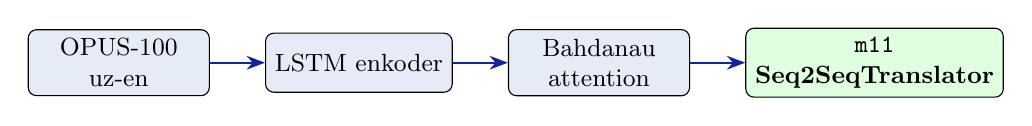
\begin{tikzpicture}[
      mod/.style={draw, fill=cnubluebg, rounded corners=3pt,
                  minimum width=2.3cm, minimum height=0.75cm,
                  font=\small, align=center},
      fin/.style={draw, fill=green!12, rounded corners=3pt,
                  minimum width=2.5cm, minimum height=0.75cm,
                  font=\small\bfseries, align=center},
      arr/.style={-{Stealth}, thick, color=cnublue}
  ]
    \node[mod] (op) {OPUS-100\\ uz-en};
    \node[mod, right=0.7cm of op]  (en) {LSTM enkoder};
    \node[mod, right=0.7cm of en]  (at) {Bahdanau\\ attention};
    \node[fin, right=0.7cm of at]  (m11) {\texttt{m11}\\ Seq2SeqTranslator};
    \draw[arr] (op)--(en); \draw[arr] (en)--(at); \draw[arr] (at)--(m11);
  \end{tikzpicture}
  \end{center}
  \vspace{5pt}
  \begin{columns}[T]
    \begin{column}{0.50\textwidth}
      \textbf{P11 da qurasiz:}\\[3pt]
      \small
      \begin{itemize}\setlength\itemsep{2pt}
        \item \texttt{m11 Seq2SeqTranslator}: enkoder-dekoder $+$ attention
        \item OPUS-100 uz-en da o'qitish, BLEU baho
        \item Attention vaznlari $\alpha$ ni tekshirish
      \end{itemize}
    \end{column}
    \begin{column}{0.46\textwidth}
      \textbf{Birinchi assert (bu slayd [I3]):}\\[4pt]
      \small\ttfamily
      assert np.allclose(\\
      \phantom{xx}alpha, [0.245,0.090,0.665],\\
      \phantom{xx}atol=1e-3)\\[4pt]
      \normalfont\footnotesize\color{halfgray}
      \textit{\# Ma'ruza L11 [I3]-slayd bilan}\\
      \textit{\# solishtiring (attention softmax)}
    \end{column}
  \end{columns}
\end{frame}

% ----------------------------------------------------------------
% [R] ADABIYOTLAR
% ----------------------------------------------------------------
\begin{frame}{Adabiyotlar}
  \begin{enumerate}\small\setlength\itemsep{5pt}
    \item Bahdanau, D., Cho, K., Bengio, Y.\ (2015). \textit{Neural Machine Translation
          by Jointly Learning to Align and Translate.} ICLR 2015.
    \item Sutskever, I., Vinyals, O., Le, Q.\ (2014). \textit{Sequence to Sequence
          Learning with Neural Networks.} NeurIPS 27.
    \item Luong, M., Pham, H., Manning, C.\ (2015). \textit{Effective Approaches to
          Attention-based NMT.} EMNLP 2015. (Dot-product attention.)
    \item Papineni, K., va boshq.\ (2002). \textit{BLEU: a Method for Automatic
          Evaluation of MT.} ACL 2002.
    \item \texttt{nltk.translate.bleu\_score} hujjatlari.
  \end{enumerate}
\end{frame}

% ================================================================
% [S] ILOVALAR (appendix --- slayd soniga kirmaydi)
% ================================================================
\appendix

\begin{frame}{Ilova S1: additive vs dot-product attention}
  \small
  Energiya $e_{t,i}$ ni hisoblashning ikki keng tarqalgan usuli:
  \begin{itemize}\setlength\itemsep{2pt}
    \item \textbf{Additive} (Bahdanau): $e_{t,i}=\mathbf{v}_a^\top\tanh(W_a s_{t-1}+U_a h_i)$
          --- kichik MLP.
    \item \textbf{Dot-product} (Luong): $e_{t,i}=s_{t-1}^\top h_i$ --- tezroq,
          parametrsiz.
  \end{itemize}
  \bunda{Transformer (L12) masshtablangan dot-product ishlatadi:
  $e=\tfrac{q^\top k}{\sqrt{d}}$ --- $\sqrt{d}$ gradientni barqarorlashtiradi.}
\end{frame}

\begin{frame}{Ilova S2: to'liq BLEU (n-gram va clipping)}
  \small
  To'liq BLEU bir nechta $n$ uchun aniqlikni geometrik o'rtachalaydi:
  $$ \mathrm{BLEU} = \mathrm{BP}\cdot\exp\!\Big(\tfrac{1}{N}\sum_{n=1}^{N}\ln p_n\Big),
     \quad N=4 \ \text{(odatda)} $$
  \bunda{\textbf{clipping}: bir so'z reference da necha marta bo'lsa, shuncha marta
  hisoblanadi (takroriy so'z bilan aldashni oldini oladi).}
  \vspace{4pt}

  Misol: hypothesis \texttt{the the the} --- clippingsiz $p_1{=}1$; clipping bilan
  reference da \texttt{the} bir marta bo'lsa, $p_1{=}1/3$.
\end{frame}

\end{document}
